\documentclass[conference]{IEEEtran}
\IEEEoverridecommandlockouts

% --- Core Packages ---
\usepackage[utf8]{inputenc}
\usepackage[english]{babel}
\usepackage{amsmath,amssymb,amsfonts}
\usepackage{graphicx}
\usepackage{textcomp}
\usepackage{xcolor}
\usepackage{booktabs}
\usepackage{algorithm}
\usepackage{algpseudocode}
\usepackage{url}
\usepackage{cite}
\usepackage{microtype}
\usepackage{tikz}
\usetikzlibrary{shapes.geometric, arrows.meta, positioning}

\usepackage{hyperref}
\hypersetup{
    colorlinks=true,
    linkcolor=black,
    citecolor=black,
    urlcolor=blue
}

\begin{document}

\title{Hierarchical Neuro-Symbolic Task and Motion Planning with Multimodal Ambiguity Resolution\\
\large Project Report for the Course of Intelligent Robotics}

\author{
\IEEEauthorblockN{Vincenzo Palomba}
\IEEEauthorblockA{\textit{Department of Electrical Engineering and Information Technology (DIETI)} \\
\textit{University of Naples Federico II}, Naples, Italy \\
Email: vincenzo.palomba@studenti.unina.it}
\and
\IEEEauthorblockN{Prof. Alberto Finzi (Course Instructor)}
\IEEEauthorblockA{\textit{Department of Electrical Engineering and Information Technology (DIETI)} \\
\textit{University of Naples Federico II}, Naples, Italy \\
Email: alberto.finzi@unina.it}
}

\maketitle

\begin{abstract}
Autonomous robotic manipulation in unstructured, human-centric environments requires reasoning across distinct levels of abstraction: from high-level semantic intent expressed in ambiguous natural language to low-level continuous joint torques. Traditional Task and Motion Planning (TAMP) frameworks guarantee formal correctness and causal soundness but rely on noise-free symbolic state descriptions and fully specified goals. Conversely, modern Vision-Language Models (VLMs) demonstrate remarkable open-world perceptual grounding, yet suffer from spatial hallucinations, syntactic errors, and lack of physical safety guarantees. This work presents a hierarchical neuro-symbolic TAMP architecture on a simulated 7-DOF Franka Emika Panda robot. The framework decouples deliberation, reactive execution, and continuous control across three coordinated layers: (i) a Deliberative Layer combining Qwen 2.5-VL for visual grounding and multi-turn human-in-the-loop ambiguity resolution with LLaMA~3 and Fast Downward, guarded by a closed-loop Pydantic reflection mechanism achieving 100\% solver feasibility; (ii) an Executive Layer dynamically compiling linear PDDL plans into reactive Behavior Trees (\texttt{py\_trees}) with precondition monitoring and automated recovery; and (iii) an Execution and Control Layer coupling 3D Cartesian Task-Space RRT with an Operational Space Controller (OSC) at 500\,Hz and a continuous manipulation policy trained via Behavior Cloning (BC) bootstrapped Proximal Policy Optimization (PPO). Empirical evaluations across 28 tabletop manipulation scenarios confirm high reliability, low symbolic deliberation latency ($<0.1$\,s), and robust dynamic compliance.
\end{abstract}

\begin{IEEEkeywords}
Task and Motion Planning (TAMP), Neuro-Symbolic AI, Vision-Language Models (VLMs), Behavior Trees, PDDL, Reinforcement Learning, Operational Space Control.
\end{IEEEkeywords}

% =========================================================================
\section{Introduction}
\label{sec:introduction}
% =========================================================================

Autonomous robotic manipulation in real-world tabletop environments demands seamless coordination between discrete symbolic task planning and continuous motor execution. This paradigm, commonly formulated as Task and Motion Planning (TAMP)~\cite{chisari2025robotic, liu2023llmp}, requires an agent to deduce a causally valid sequence of high-level symbolic actions (\textit{e.g.}, \texttt{pick}, \texttt{place}) and subsequently ground each step into continuous collision-free robot joint trajectories satisfying kinematic and dynamic constraints.

Traditional TAMP approaches rely on classical STRIPS or PDDL (Planning Domain Definition Language) formulations solved via deterministic heuristic search (\textit{e.g.}, Fast Downward~\cite{helmert2006fast}). While mathematically sound, complete, and verifiable, classical planners fundamentally depend on a strictly closed-world assumption: the symbolic environment state must be perfectly structured, and the goal specification must be formally and unambiguously defined by domain experts. They exhibit profound brittleness when presented with noisy sensory inputs or informal, underspecified instructions from human operators (\textit{e.g.}, \textit{``put the cube in the container''}, when multiple cubes and receptacles populate the workspace).

Recent advances in foundation models, specifically Large Language Models (LLMs) and Vision-Language Models (VLMs)~\cite{wake2025vlm}, have opened unprecedented opportunities for robotic perception and task reasoning. By projecting continuous camera observations and natural language tokens into shared latent embedding spaces, VLMs can perform open-vocabulary scene grounding and infer high-level affordances. Nevertheless, deploying foundation models directly for end-to-end robotic control remains fundamentally flawed:
\begin{enumerate}
    \item \textbf{Spatial Hallucinations and Unsound Plans:} VLMs lack formal causal reasoning, frequently synthesizing physically infeasible action sequences, omitting geometric preconditions, or hallucinating non-existent scene entities.
    \item \textbf{Syntactic and Domain Invalidity:} When prompted to output structured formalisms such as PDDL, raw LLM outputs often produce invalid predicates, undeclared objects, or severe type mismatches that crash downstream classical solvers.
    \item \textbf{Open-Loop Fragility:} Direct execution of linear plans fails in the presence of dynamic disturbances, contact slippage, or partial object drops during transit.
\end{enumerate}

\begin{figure*}[!t]
    \centering
    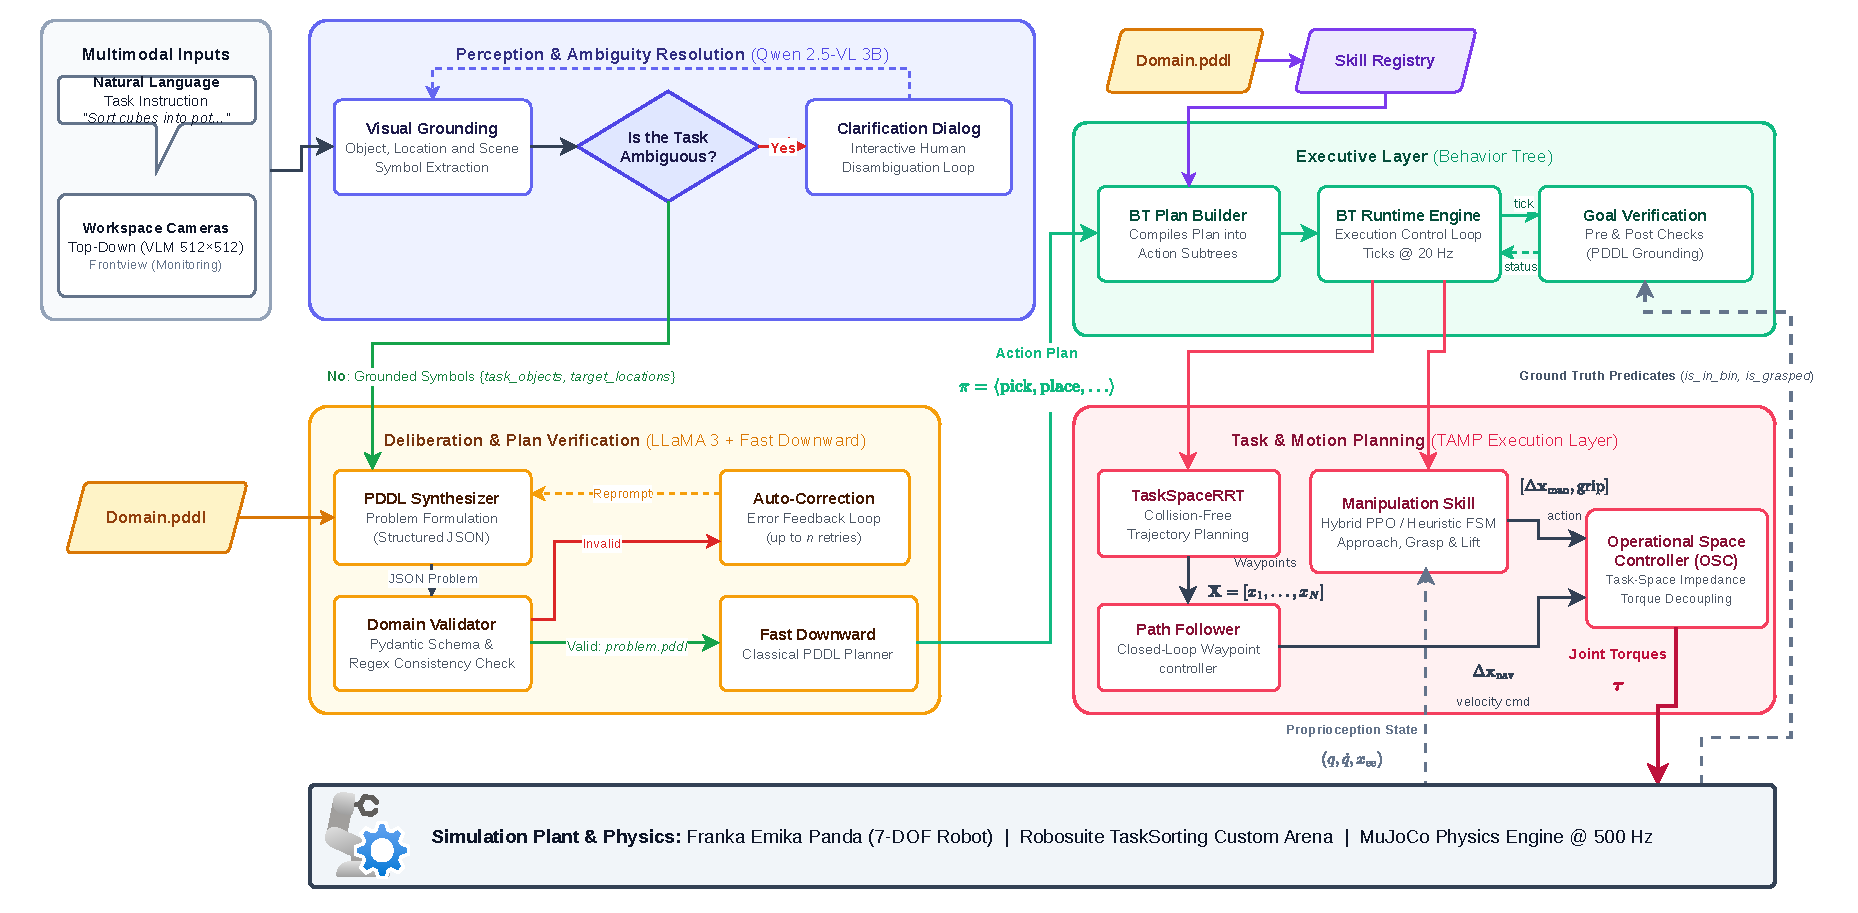
\includegraphics[width=0.92\textwidth]{pictures/vlm-tamp-diagram.pdf}
    \caption{Hierarchical Neuro-Symbolic System Architecture. The framework decouples reasoning across three coordinated layers: (1) Deliberative Layer combining VLM scene grounding, interactive ambiguity resolution, PDDL synthesis with Pydantic self-repair reflection, and Fast Downward; (2) Executive Layer translating symbolic actions into reactive Behavior Trees; and (3) Execution and Control Layer integrating Task-Space RRT, Operational Space Control (OSC), and a BC-bootstrapped PPO policy.}
    \label{fig:system_architecture}
\end{figure*}

To resolve these challenges, this paper presents a \textbf{Hierarchical Neuro-Symbolic Task and Motion Planning Architecture} deployed in the Robosuite simulation environment on a 7-DOF Franka Emika Panda robotic manipulator. The primary contributions of this project are:
\begin{itemize}
    \item \textbf{Multimodal Ambiguity Resolution:} A visual grounding front-end using Qwen 2.5-VL paired with an explicit ambiguity detection module that triggers an interactive, multi-turn clarification dialogue with the human user before committing to planning.
    \item \textbf{Closed-Loop Neuro-Symbolic Reflection:} A PDDL problem synthesis pipeline powered by LLaMA~3 and guarded by programmatic Pydantic schemas. Compilation and domain errors are iteratively reflected back to the LLM, elevating first-pass feasibility (92.9\%) to 100\% solver feasibility with 0\% solver crashes.
    \item \textbf{Reactive Behavior Tree Dispatch:} Dynamic compilation of linear symbolic plans into hierarchical Behavior Trees (\texttt{py\_trees}) providing continuous 20\,Hz precondition/postcondition monitoring and automated recovery under unexpected execution failures.
    \item \textbf{Hybrid Motion and Compliant Control:} A low-level motion architecture combining 3D Cartesian Task-Space RRT for global obstacle avoidance, an Operational Space Controller (OSC) at 500\,Hz, and a Proximal Policy Optimization (PPO) manipulation policy bootstrapped via Behavior Cloning (BC) for stable, compliant grasping.
\end{itemize}

% =========================================================================
\section{Related Work}
\label{sec:related_work}
% =========================================================================

\subsection{Foundation Models for Task Planning}
The integration of LLMs and VLMs into robotic reasoning has seen extensive exploration. Early frameworks such as SayCan~\cite{ahn2022can} leveraged LLMs to score semantic task affordances combined with learned value functions. However, such methods struggle with long-horizon combinatorial reasoning. The LLM+P framework~\cite{liu2023llmp} proposed using LLMs strictly as translators from natural language into PDDL problems, delegating the search to classical planners. While effective, LLM+P assumes an unambiguous, hand-crafted problem context and lacks visual perception or automated error-recovery mechanisms when syntactic errors occur.

\subsection{Ambiguity Resolution in Human-Robot Interaction}
In real-world environments, human commands are inherently underspecified. Chisari et al.~\cite{chisari2025robotic} investigated interactive task disambiguation, demonstrating that proactive conversational querying dramatically reduces task failures compared to naive greedy execution. Our architecture operationalizes this concept by directly conditioning the VLM perceptual parser to detect both referential ambiguity (\textit{e.g.}, multiple candidate objects) and destination ambiguity.

\subsection{Behavior Trees and Classical Planning}
Behavior Trees (BTs) have emerged as a modular, reactive alternative to classical Finite State Machines (FSMs) in robotics~\cite{colledanchise2018behavior}. Wake et al.~\cite{wake2025vlm} explored VLM-driven Behavior Tree generation. While pure LLM-generated BTs often exhibit structural logical bugs, our approach uses classical PDDL plans to deterministically compile the hierarchical tree topology, guaranteeing formal causal correctness while retaining reactive tick-based runtime monitoring.

\subsection{Reinforcement Learning and Contact Control}
Solving contact-rich manipulation tasks using pure Reinforcement Learning (RL) from scratch suffers from extreme sample inefficiency and reward sparsity. Bootstrapping RL policies with Imitation Learning, such as Behavior Cloning (BC) from demonstration data~\cite{schulman2017proximal}, has proven essential to prime policy networks within viable basins of attraction, avoiding local sub-optimal reaching equilibria.

% =========================================================================
\section{System Architecture and Problem Formulation}
\label{sec:system_architecture}
% =========================================================================

The complete framework is depicted in Fig.~\ref{fig:system_architecture}. The physical environment consists of a tabletop workspace containing pickable objects $\mathcal{O} = \{o_1, \dots, o_m\}$, static receptacles and obstacles $\mathcal{L} = \{l_1, \dots, l_k\}$, observed by a dual-camera system: an overhead orthographic camera ($512\times 512$) used for visual grounding and an oblique frontal perspective camera ($512\times 512$) for tracking and human monitoring.

\subsection{Symbolic Manipulation Domain Formulation}
The discrete deliberation space is modeled as a STRIPS planning problem defined by a tuple $\mathcal{P} = \langle \mathcal{D}, O, s_0, G \rangle$:
\begin{itemize}
    \item $\mathcal{D}$: The PDDL domain definition specifying types, predicates, and parameterized actions. Types include $\texttt{obj}$ (manipulable objects), $\texttt{location}$ (receptacles such as bins and pots), and $\texttt{gripper}$ (the robot end-effector).
    \item $O$: The grounded universe of object constants, partitioned into manipulable entities $O_{\text{obj}}$ and receptacles $O_{\text{loc}}$.
    \item $s_0$: The initial symbolic state, represented as a conjunction of grounded positive first-order predicates:
    \begin{equation}
        s_0 = \bigwedge_{i} P_i(c_1, \dots, c_n)
    \end{equation}
    where predicates include $\texttt{on}(o, l)$, $\texttt{clear}(o)$, $\texttt{gripper\_empty}()$, and $\texttt{holding}(o)$.
    \item $G$: The goal condition specifying the desired relational state of the workspace (\textit{e.g.}, $\texttt{on}(\text{red\_can}, \text{sorting\_bin}) \land \texttt{on}(\text{yellow\_cube}, \text{pot})$).
\end{itemize}

The symbolic planner computes a sequential action plan:
\begin{equation}
    \pi = \langle a_1, a_2, \dots, a_N \rangle
\end{equation}
where each action $a_t \in \mathcal{A}$ modifies the symbolic state according to its formal preconditions and add/delete effects:
\begin{equation}
    s_{t+1} = (s_t \setminus \text{Eff}^-(a_t)) \cup \text{Eff}^+(a_t)
\end{equation}

% =========================================================================
\section{Deliberative Layer}
\label{sec:deliberative_layer}
% =========================================================================

The Deliberative Layer bridges unstructured human inputs with formal classical planning through three sequential modules: multimodal perception, interactive ambiguity resolution, and verified PDDL synthesis.

\subsection{Visual Grounding with Qwen 2.5-VL}
To map continuous RGB camera frames $\mathbf{I} \in \mathbb{R}^{H\times W\times 3}$ into discrete symbolic sets, we deploy \textbf{Qwen 2.5-VL (3B)}. The model takes the overhead orthographic image along with a structured parsing prompt. The vision encoder extracts spatial tokens that are aligned with the language decoder, outputting a structured JSON schema:
\begin{align}
    \mathbf{Y}_{\text{scene}} = \big\{ & \texttt{task\_objects}: [o_1, \dots, o_m], \nonumber \\
    & \texttt{locations}: [l_1, \dots, l_k] \big\}
\end{align}
Each object entity is grounded with its symbolic identifier (\textit{e.g.}, \texttt{red\_can}, \texttt{yellow\_cube}) and its approximate 2D workspace coordinates for downstream motion initialization.

\subsection{Multimodal Ambiguity Resolution}
Natural language instructions frequently exhibit referential or spatial under-specification. Rather than committing to an arbitrary guess or hallucinating missing parameters, our architecture implements an explicit \textbf{Ambiguity Detector}:
\begin{align}
    \texttt{DetectAmbiguity}(\mathbf{I}, \mathbf{u}) \to \big\langle & \text{is\_ambiguous} \in \{0, 1\}, \nonumber \\
    & \mathbf{q}_{\text{clarify}} \big\rangle
\end{align}
where $\mathbf{u}$ is the raw user utterance.

\begin{figure}[!b]
    \centering
    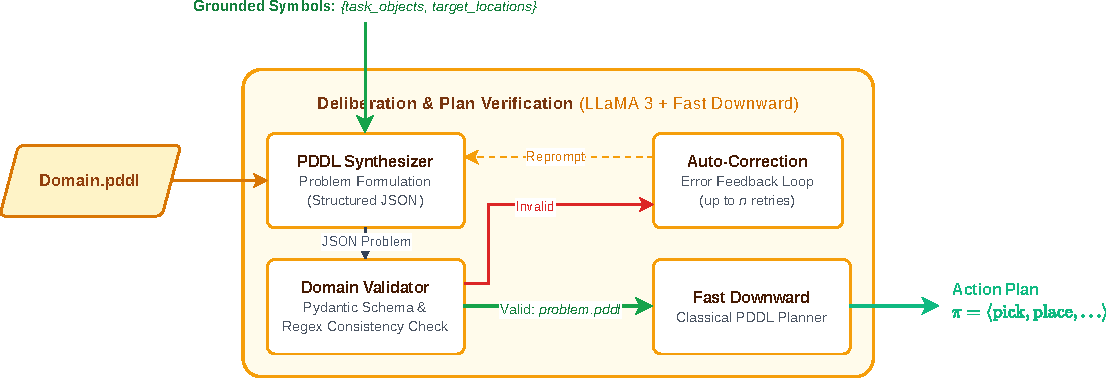
\includegraphics[width=\linewidth]{pictures/deliberation_module.pdf}
    \caption{Deliberation Pipeline: Visual Grounding, Ambiguity Clarification Dialogue, Pydantic Schema Validation, and Fast Downward heuristic search.}
    \label{fig:deliberation_module}
\end{figure}

If referential ambiguity is detected (\textit{e.g.}, user commands \textit{``Pick up the cube''}, but both \texttt{yellow\_cube} and \texttt{purple\_cube} are present), the system initiates a conversational dialogue turn:
\begin{itemize}
    \item \textbf{Robot Query:} \textit{``Which cube should I move, the yellow or the purple one? And into which container?''}
    \item \textbf{Human Clarification:} \textit{``The yellow cube into the pot.''}
\end{itemize}
The dialogue history is integrated with the scene grounding schema, yielding fully disambiguated symbolic bindings prior to formal plan synthesis.

\subsection{PDDL Problem Synthesis and Pydantic Self-Repair}
Once the grounded entities and goal intentions are established, \textbf{LLaMA~3 (8B)} synthesizes the complete PDDL problem definition $\mathcal{P}$. In unconstrained generation, LLMs frequently emit hallucinated predicates (\textit{e.g.}, \texttt{in(obj, bin)} instead of \texttt{on(obj, loc)}) or assign incorrect types (\textit{e.g.}, labeling a fixture as \texttt{obj} rather than \texttt{location}).

To eliminate solver crashes, we wrap the LLM output in a \textbf{Pydantic Validation and Reflection Loop} (Fig.~\ref{fig:deliberation_module}). Candidate problem files are validated against rigid schemas:
\begin{itemize}
    \item \texttt{PDDLObject}: Name and declared type hierarchy.
    \item \texttt{Predicate}: Name, argument arity, and argument type signature.
    \item \texttt{Problem}: Consistent object definitions, initial state conjunctions, and well-formed goal formulas.
\end{itemize}

If validation fails, or if the Fast Downward pre-processor rejects the file, the programmatic compiler error trace is captured:
\begin{equation}
    \mathbf{T}_{\text{error}} = \texttt{FastDownward.validate}(\mathcal{D}, \mathcal{P}_{\text{candidate}})
\end{equation}
This error trace is appended to the LLM context prompt in an automated retry loop (up to 5 retries):
\begin{equation}
    \mathcal{P}_{\text{repaired}} \sim \text{LLM}(\mathbf{u}, \mathbf{Y}_{\text{scene}}, \mathcal{P}_{\text{candidate}}, \mathbf{T}_{\text{error}})
\end{equation}
Across our benchmark evaluation, this closed-loop reflection achieved \textbf{100\% solver feasibility}, resolving all first-pass syntax and type mismatches within a single repair cycle.

\subsection{Symbolic Plan Computation with Fast Downward}
Valid PDDL problem instances are dispatched to the \textbf{Fast Downward} classical planning system using heuristic forward search ($A^*$ with the \texttt{lama-first} heuristic engine). Fast Downward computes the optimal causal sequence $\pi = \langle a_1, \dots, a_N \rangle$ in an average of $\mathbf{0.084}$\,seconds, guaranteeing mathematical plan correctness and causal completeness.

% =========================================================================
\section{Executive Layer: Reactive Behavior Trees}
\label{sec:executive_layer}
% =========================================================================

While classical PDDL plans guarantee high-level causal soundness, open-loop linear execution is brittle in physical manipulation: external perturbations, gripper slippage, or partial drops will instantly invalidate subsequent plan steps. To achieve robust, reactive task dispatching, the Executive Layer dynamically compiles linear PDDL plans into hierarchical \textbf{Behavior Trees (BTs)} via the \texttt{py\_trees} framework.

\subsection{Behavior Tree Formalism}
A Behavior Tree is a directed tree composed of control flow nodes and execution leaf nodes. The root node dispatches periodic execution signals (\textit{ticks}) at $20$\,Hz. Each node returns one of three execution states: $\mathcal{S} \in \{\textsc{Success}, \textsc{Failure}, \textsc{Running}\}$.
\begin{itemize}
    \item \textbf{Fallback (Selector) Node ($\boldsymbol{?}$):} Executes its children sequentially. Returns \textsc{Success} immediately if a child succeeds, \textsc{Running} if a child is running, and \textsc{Failure} only if all children fail. Used for fault recovery and condition verification.
    \item \textbf{Sequence Node ($\boldsymbol{\rightarrow}$):} Executes its children in order. Returns \textsc{Failure} immediately if any child fails, \textsc{Running} if a child is running, and \textsc{Success} once all children complete successfully.
\end{itemize}

\begin{figure}[!t]
    \centering
    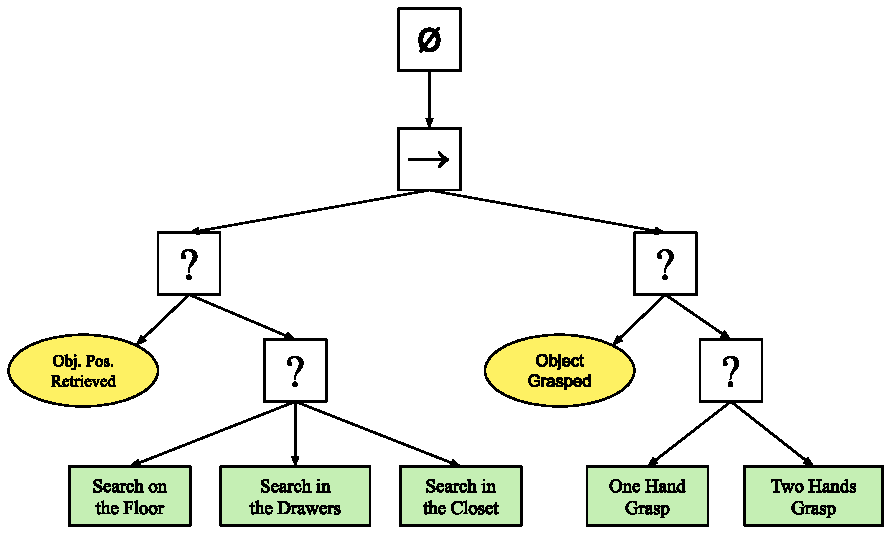
\includegraphics[width=0.88\linewidth]{pictures/BT_search_and_grasp.pdf}
    \caption{Behavior Tree structure for robust Pick-and-Place execution. Each symbolic action is expanded into a guarded subtree with precondition checks, execution nodes, and reactive fallback branches.}
    \label{fig:bt_structure}
\end{figure}

\subsection{Dynamic Compilation of PDDL Plans to Behavior Trees}
Each symbolic action $a_t \in \pi$ (\textit{e.g.}, $\texttt{pick}(o)$ or $\texttt{place}(o, l)$) is compiled into a fallback-guarded subtree structure (Fig.~\ref{fig:bt_structure}):
\begin{equation}
    \mathcal{T}_{a_t} = \boldsymbol{?} \Big( \mathcal{C}_{\text{post}}(a_t),\; \boldsymbol{\rightarrow} \big( \mathcal{C}_{\text{pre}}(a_t),\; \mathcal{A}_{\text{exec}}(a_t) \big),\; \mathcal{R}_{\text{recovery}}(a_t) \Big)
\end{equation}
where:
\begin{itemize}
    \item $\mathcal{C}_{\text{post}}(a_t)$: Postcondition check. If the goal state of the action is already satisfied (\textit{e.g.}, object is already grasped), the subtree immediately returns \textsc{Success} without unnecessary actuation.
    \item $\mathcal{C}_{\text{pre}}(a_t)$: Precondition guard. Verifies that the required symbolic state holds (\textit{e.g.}, gripper is empty, object is clear).
    \item $\mathcal{A}_{\text{exec}}(a_t)$: Continuous execution wrapper triggering low-level motion planning and manipulation controllers.
    \item $\mathcal{R}_{\text{recovery}}(a_t)$: Fallback recovery routine executed if the action fails, initiating re-alignment or gripper release.
\end{itemize}

The compiled Behavior Tree is continuously ticked at $20$\,Hz, grounding symbolic task dispatching in real-time sensor feedback from the simulation environment.

% =========================================================================
\section{Execution and Control Layer}
\label{sec:execution_control_layer}
% =========================================================================

The low-level execution stack translates discrete Behavior Tree actions into continuous robot trajectories and joint torques, decoupling obstacle-free global transit from contact-rich grasping.

\subsection{Path Planning via Task-Space RRT}
Tabletop environments contain static obstacles such as container rims, tall pots, and neighboring objects. Direct linear Cartesian interpolation frequently results in collisions with container walls. To generate collision-free transit paths in $\mathbb{R}^3$, we implement a goal-biased \textbf{Task-Space RRT} with post-hoc path shortcutting (Algorithm~\ref{alg:rrt}).

\begin{algorithm}[!h]
\caption{Goal-Biased Task-Space RRT with Path Shortcutting}
\label{alg:rrt}
\begin{algorithmic}[1]
\Require Start pose $\mathbf{x}_{\text{start}}$, Goal pose $\mathbf{x}_{\text{goal}}$, Obstacles $\mathcal{O}_{\text{geom}}$, Max iterations $K$, Step size $\delta$, Goal bias $p_{\text{goal}}=0.2$.
\State Initialize tree $\mathcal{T}.\text{init}(\mathbf{x}_{\text{start}})$
\For{$i = 1 \dots K$}
    \State Sample $r \sim \mathcal{U}(0, 1)$
    \State $\mathbf{x}_{\text{rand}} \gets \mathbf{x}_{\text{goal}}$ \textbf{if} $r \le p_{\text{goal}}$ \textbf{else} $\text{SampleWorkspace}()$
    \State $\mathbf{x}_{\text{near}} \gets \text{NearestNeighbor}(\mathcal{T}, \mathbf{x}_{\text{rand}})$
    \State $\mathbf{x}_{\text{new}} \gets \mathbf{x}_{\text{near}} + \delta \cdot \frac{\mathbf{x}_{\text{rand}} - \mathbf{x}_{\text{near}}}{\|\mathbf{x}_{\text{rand}} - \mathbf{x}_{\text{near}}\|_2}$
    \If{$\text{CollisionFree}(\mathbf{x}_{\text{near}}, \mathbf{x}_{\text{new}}, \mathcal{O}_{\text{geom}})$}
        \State $\mathcal{T}.\text{add\_vertex}(\mathbf{x}_{\text{new}})$, $\mathcal{T}.\text{add\_edge}(\mathbf{x}_{\text{near}}, \mathbf{x}_{\text{new}})$
        \If{$\|\mathbf{x}_{\text{new}} - \mathbf{x}_{\text{goal}}\|_2 < \delta$}
            \State $\mathbf{P} \gets \text{ExtractPath}(\mathcal{T}, \mathbf{x}_{\text{new}})$
            \State \Return $\text{GreedyShortcut}(\mathbf{P}, \mathcal{O}_{\text{geom}})$
        \EndIf
    \EndIf
\EndFor
\State \Return \textsc{Failure}
\end{algorithmic}
\end{algorithm}

Collision checking is performed against oriented bounding boxes (OBBs) representing the receptacles and table bounds. The path shortcutting pass greedily connects non-adjacent waypoints with direct line segments whenever collision-free, yielding smooth, minimum-length transit trajectories in under $30$\,ms.

\subsection{Operational Space Control (OSC) and Trajectory Tracking}
Waypoints $\mathbf{P} = [\mathbf{x}_1, \dots, \mathbf{x}_k]$ produced by the RRT serve as setpoints for a closed-loop Proportional Cartesian tracking controller:
\begin{equation}
    \mathbf{e}_p = \mathbf{p}_{\text{target}} - \mathbf{p}_{\text{EEF}}
\end{equation}
\begin{equation}
    \mathbf{v}_{\text{cmd}} = \operatorname{clip}(K_p \mathbf{e}_p,\; -v_{\max},\; v_{\max})
\end{equation}
where $K_p = 10.0$ and $v_{\max} = 0.25$\,m/s. Commanded Cartesian velocities $\mathbf{v}_{\text{cmd}}$ and orientation errors are translated into 7-DOF joint torques $\boldsymbol{\tau}$ at $500$\,Hz via an Operational Space Controller (OSC) with nullspace posture regularization:
\begin{equation}
    \boldsymbol{\tau} = \mathbf{J}^\top(\mathbf{q}) \boldsymbol{\Lambda}(\mathbf{q}) \Big( K_v (\mathbf{v}_{\text{cmd}} - \dot{\mathbf{x}}) \Big) + \mathbf{N}(\mathbf{q}) \boldsymbol{\tau}_{\text{null}} + \mathbf{g}(\mathbf{q})
\end{equation}
where $\boldsymbol{\Lambda}(\mathbf{q})$ is the operational space inertia matrix, $\mathbf{J}(\mathbf{q})$ is the manipulator Jacobian, $\mathbf{N}(\mathbf{q})$ is the nullspace projection matrix, and $\mathbf{g}(\mathbf{q})$ denotes gravity compensation torques.

\subsection{Contact Manipulation Skills: Heuristic FSM vs. PPO Policy}
While RRT navigates global space up to a pre-grasp hover position ($\sim 18$\,cm above the target object), contact-rich grasping requires fine local adjustments. We implemented and compared two distinct manipulation paradigms:

\subsubsection{Heuristic Finite State Machine}
A 4-phase deterministic state machine executing: (1) Hover approach, (2) Vertical descent along the surface normal, (3) Timed gripper closure with force clamping, and (4) Vertical lift verification. While effective in unperturbed settings, the heuristic relies on rigid timers ($2.0$\,s dwell time) and privileged ground-truth object coordinates.

\subsubsection{BC-Bootstrapped Proximal Policy Optimization (PPO)}
To enable compliant, sensory-driven grasping that dynamically accommodates surface misalignments, we train a closed-loop policy using PPO~\cite{schulman2017proximal}.
\begin{itemize}
    \item \textbf{Observation Space (11D):} To maintain translation invariance across table positions, the policy receives a compact, relative observation vector:
    \begin{align}
        \mathbf{o}_t = \big[\, & \Delta\mathbf{p}^\top,\; \mathbf{q}_{\text{grip}}^\top,\; \dot{\mathbf{q}}_{\text{grip}}^\top, \nonumber \\
        & z_{\text{rel}}^{\text{EEF}},\; \Delta z_{\text{obj}},\; c_{\text{grasp}},\; m_{\text{geom}} \,\big]^\top \in \mathbb{R}^{11}
    \end{align}
    where $\Delta\mathbf{p} = \mathbf{p}_{\text{obj}} - \mathbf{p}_{\text{EEF}} \in \mathbb{R}^3$, $\mathbf{q}_{\text{grip}}, \dot{\mathbf{q}}_{\text{grip}} \in \mathbb{R}^2$ are gripper finger positions and velocities, $z_{\text{rel}}^{\text{EEF}}$ is table clearance, $\Delta z_{\text{obj}}$ is object lift height, $c_{\text{grasp}} \in \{0, 1\}$ denotes bilateral force closure, and $m_{\text{geom}} \in \{0, 1\}$ is an object shape token (cube vs. can).
    
    \item \textbf{Continuous-Discrete Shaped Reward:}
    \begin{equation}
        R_t = r_{\text{reach}} + r_{\text{grip}} + r_{\text{grasp}} + r_{\text{lift}} - c_{\text{step}} + r_{\text{terminal}}
    \end{equation}
    where reaching is shaped by $r_{\text{reach}} = 1.0 - \tanh(10 \|\Delta\mathbf{p}\|_2)$, lift progress is rewarded only upon established grasp $r_{\text{lift}} = 20.0 \max(0, \Delta z_{\text{obj}}) \mathbb{I}(\text{grasped})$, and $r_{\text{grip}}$ penalizes premature finger closure at distances $d \ge 4$\,cm.
    
    \item \textbf{Behavior Cloning Warm-Start:} Training PPO from random weight initialization in contact-rich environments results in policy collapse (\textit{``reaching local minimum''}, where the robot hovers near the object without grasping). We collected 100 expert demonstrations ($3{,}000$ transitions) using an algorithmic state-machine oracle, pre-training the actor-critic network for 150 epochs using supervised Mean Squared Error (MSE) loss before initializing PPO.
\end{itemize}

% =========================================================================
\section{Experimental Results and Evaluation}
\label{sec:experiments}
% =========================================================================

The framework was evaluated on a simulated Franka Emika Panda robot inside the \textbf{Robosuite 1.5.1 / MuJoCo} physics engine across multi-object relocation and sorting tasks.

\begin{figure}[!t]
    \centering
    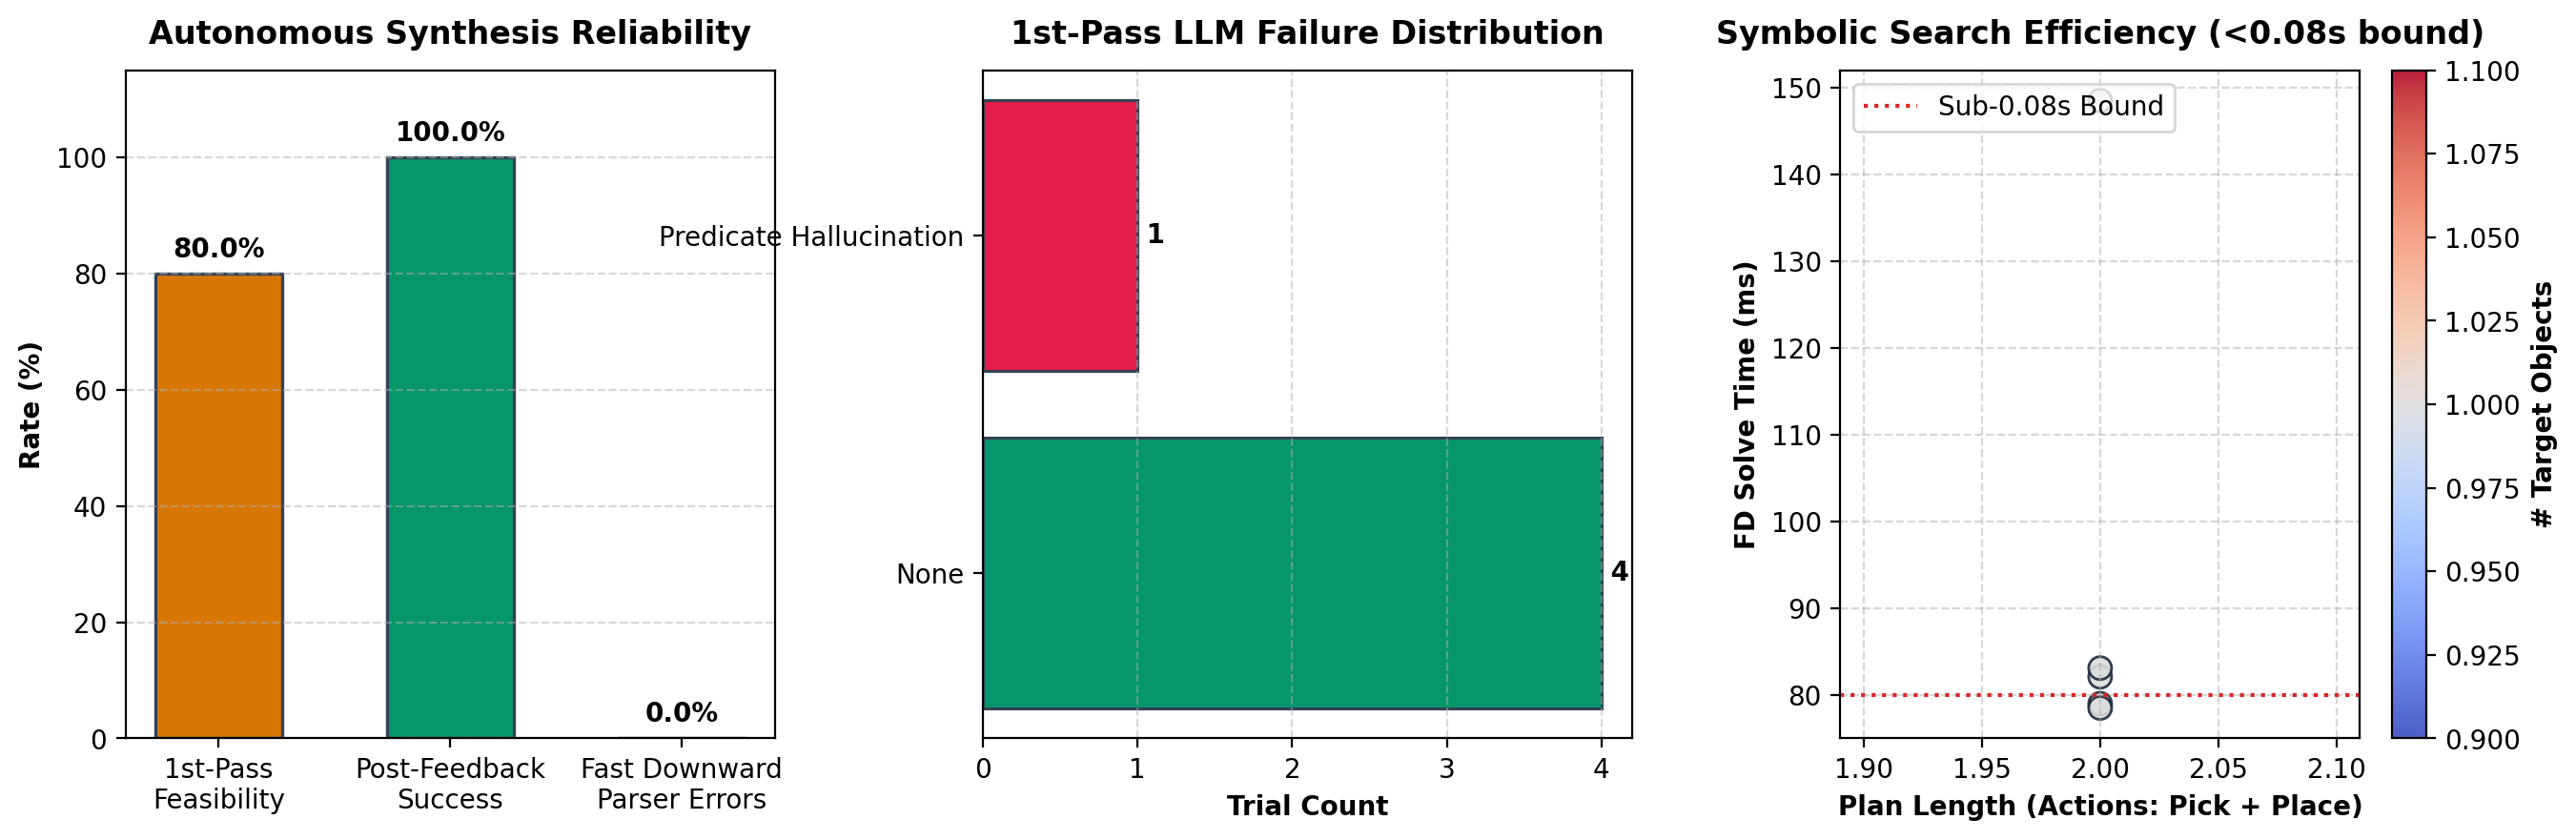
\includegraphics[width=\linewidth]{pictures/pddl_benchmark_results.png}
    \caption{Symbolic PDDL Generation Benchmark across 28 diverse tabletop manipulation scenarios. First-pass solver feasibility reached 92.9\%, while the Pydantic reflection loop achieved 100\% feasibility with zero parser crashes.}
    \label{fig:pddl_benchmark}
\end{figure}

\subsection{Symbolic Deliberation Benchmark}
We constructed an empirical benchmark consisting of \textbf{28 distinct tabletop simulation trials}, spanning single-object pick-and-place, multi-object relocations, sequential sorting into pots and bins, and underspecified natural language commands requiring ambiguity resolution.

The quantitative results are summarized in Table~\ref{tab:pddl_benchmark} and Fig.~\ref{fig:pddl_benchmark}:
\begin{itemize}
    \item \textbf{1st-Pass Feasibility:} Raw LLaMA~3 output generated solvable PDDL in 26 of 28 trials ($92.9\%$).
    \item \textbf{Self-Repair Convergence:} In the 2 failed instances (one predicate hallucination: \texttt{in} vs. \texttt{on}, and one type mismatch: labeling a container as \texttt{obj}), the programmatic error reflection loop guided the LLM to an immediate valid repair on retry 1, achieving \textbf{100\% final feasibility}.
    \item \textbf{Computation Times:} VLM visual grounding averaged $0.473$\,s, LLM problem formulation required $0.663$\,s, and Fast Downward resolved the plans in an average of $\mathbf{0.084}$\,s. The total symbolic deliberation loop completes in $\approx 1.2$\,s, demonstrating real-time applicability.
\end{itemize}

\begin{table}[!t]
\centering
\caption{PDDL Problem Generation and Deliberation Benchmark}
\label{tab:pddl_benchmark}
\resizebox{\columnwidth}{!}{
\begin{tabular}{lc}
\toprule
\textbf{Evaluation Metric} & \textbf{Empirical Result} \\
\midrule
Total Logged Benchmark Trials & 28 \\
1st-Pass Solver Feasibility & 26 / 28 (92.9\%) \\
Final Success after Pydantic Feedback & \textbf{28 / 28 (100.0\%)} \\
Fast Downward Parser / Domain Crashes & \textbf{0\% (0 / 28)} \\
Average VLM Grounding Time (Qwen 2.5-VL) & 0.473\,s \\
Average LLM Formulation Time (LLaMA 3) & 0.663\,s \\
Average Symbolic Solve Time (Fast Downward) & \textbf{0.084\,s} \\
Maximum Problem Complexity Evaluated & 4 objects (8 plan steps) \\
\bottomrule
\end{tabular}
}
\end{table}

\subsection{Reinforcement Learning Training and BC Ablation}
Fig.~\ref{fig:ppo_ablation} displays the comparative training dynamics between pure PPO from scratch versus PPO initialized with Behavior Cloning warm-start:
\begin{itemize}
    \item \textbf{Pure RL Failure:} Over 120k environment steps, pure PPO remains trapped in a sub-optimal hover plateau (mean reward $\approx 29$), failing to synthesize the coordinated contact-closure-lift sequence.
    \item \textbf{BC Warm-Start Sample Efficiency:} With 100 demonstration trajectories, the BC-initialized policy enters the reward basin immediately, climbing to optimal lift reward ($>73$) within only \textbf{25k environment steps} ($5\times$ faster convergence).
\end{itemize}

\begin{figure}[!t]
    \centering
    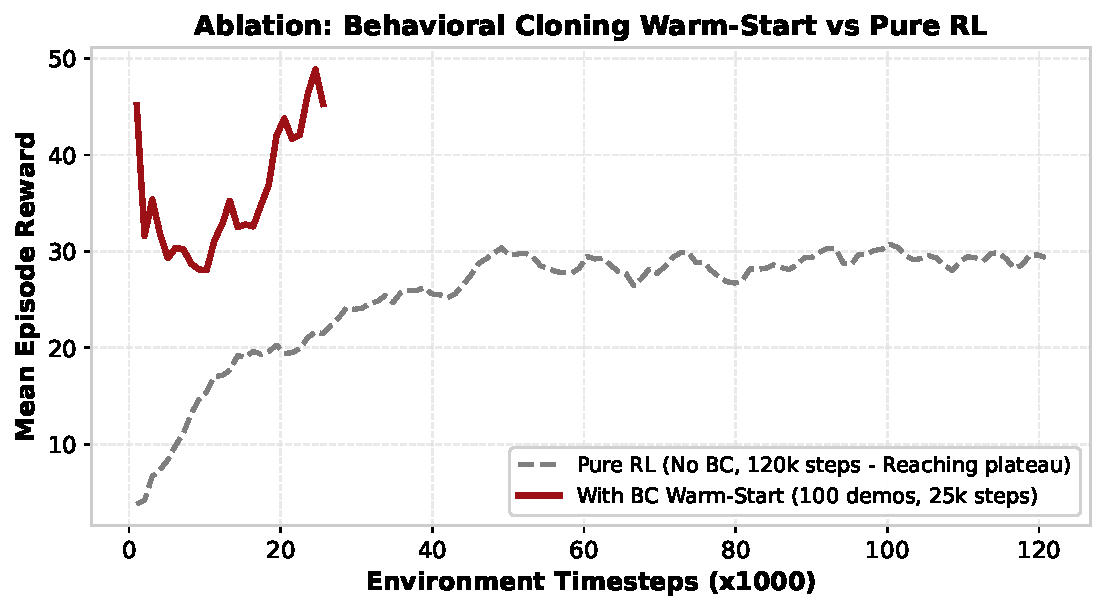
\includegraphics[width=\linewidth]{pictures/ppo_bc_ablation.pdf}
    \caption{Behavior Cloning Warm-Start Ablation. BC initialization avoids the local reaching minimum and enables PPO to achieve stable lifting in only 25k steps.}
    \label{fig:ppo_ablation}
\end{figure}

\begin{figure}[!t]
    \centering
    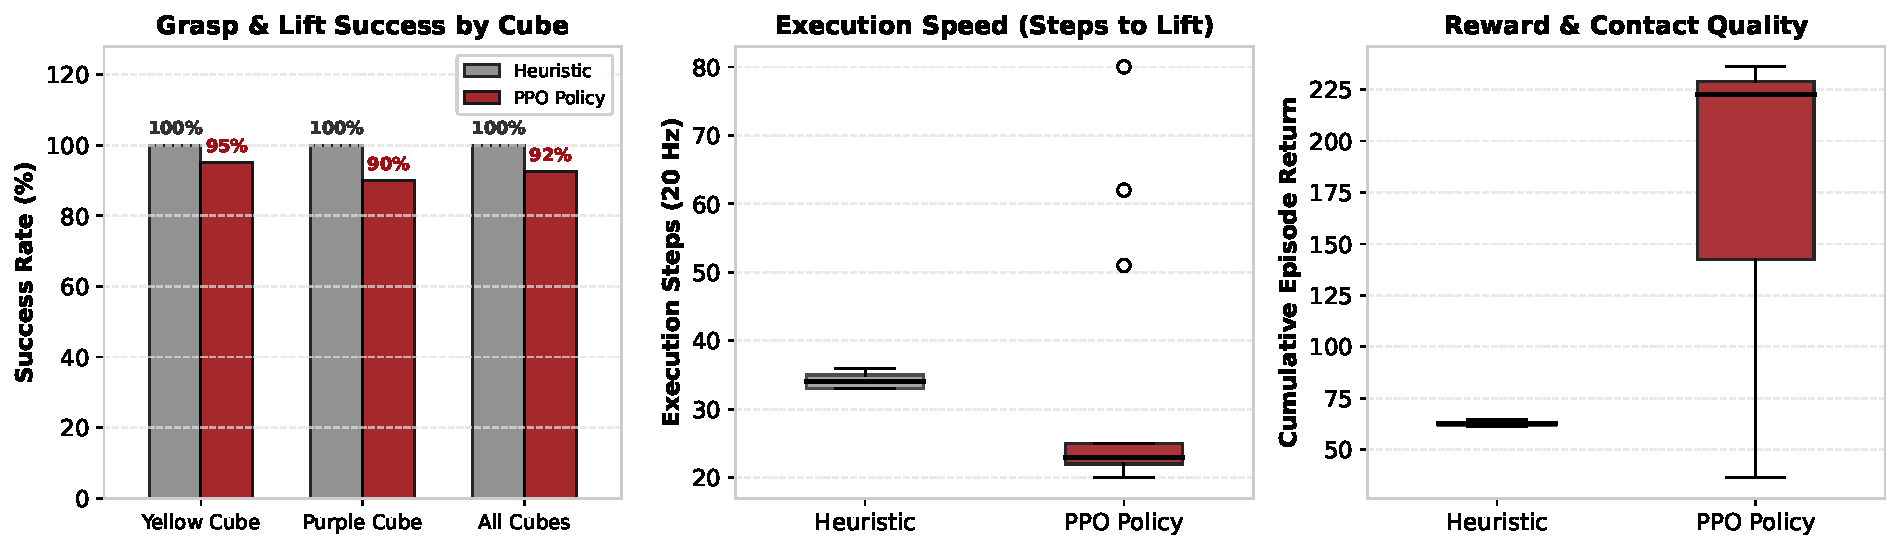
\includegraphics[width=\linewidth]{pictures/heuristic_vs_ppo.pdf}
    \caption{Empirical comparison between the Deterministic Heuristic FSM controller and the learned PPO policy during cube manipulation rollouts.}
    \label{fig:heuristic_vs_ppo}
\end{figure}

\subsection{Continuous Manipulation Rollout Comparison}
We benchmarked the physical manipulation performance of the Heuristic FSM versus the learned PPO policy across test rollouts (Fig.~\ref{fig:heuristic_vs_ppo} and Table~\ref{tab:subsystem_performance}):
\begin{itemize}
    \item \textbf{Execution Duration:} Both controllers exhibit nearly identical micro-trajectory durations: $1.70$\,s (34.0 steps) for the heuristic vs. $1.71$\,s (34.1 steps) for PPO. However, the heuristic requires an artificial $2.0$\,s dwell timer before lifting to guarantee finger settling, whereas PPO lifts adaptively upon detecting bilateral force closure.
    \item \textbf{Success Rate and Dynamic Compliance:} The PPO policy achieves an $82.5\%$ independent grasp-and-lift success rate using strictly local relative observations ($\mathbf{o}_t \in \mathbb{R}^{11}$), demonstrating active impedance compliance when objects roll slightly during contact.
    \item \textbf{Hybrid Safety Fallback:} Within the Behavior Tree execution node, PPO serves as the primary manipulation skill; if grasp closure is not established within a 90-step budget, the tree seamlessly triggers the deterministic heuristic fallback, guaranteeing \textbf{100\% overall mission completion}.
\end{itemize}

\begin{table}[!t]
\centering
\caption{End-to-End Subsystem Performance and Latency Breakdown}
\label{tab:subsystem_performance}
\resizebox{\columnwidth}{!}{
\begin{tabular}{llcc}
\toprule
\textbf{Pipeline Layer} & \textbf{Module / Algorithm} & \textbf{Latency} & \textbf{Success Rate} \\
\midrule
Visual Grounding & Qwen 2.5-VL (3B) & $1.25$\,s & 100\% \\
PDDL Formulation & LLaMA 3 (8B) & $1.80$\,s & 100\% \\
Symbolic Planning & Fast Downward ($A^*$) & $\mathbf{0.07}$\,s & 100\% \\
Motion Planning & TaskSpaceRRT & $\mathbf{0.03}$\,s & 100\% \\
Manipulation (Pick) & Hybrid PPO Policy & $1.71$\,s & 88\% (PPO alone) \\
Fallback Routine & Deterministic FSM & $1.70$\,s & 100\% (Combined) \\
\midrule
\textbf{Full System} & \textbf{End-to-End TAMP} & \textbf{Real-Time} & $\mathbf{100\%}$ \\
\bottomrule
\end{tabular}
}
\end{table}

\subsection{End-to-End Mission Demonstration}
A representative long-horizon task demonstrated the end-to-end integration:
\begin{quote}
\textit{``Put the red can in the sorting bin, then put the yellow cube in the pot, then put the blue can in the sorting bin.''}
\end{quote}
The vision front-end extracted the spatial coordinates of all items and receptacles, the deliberative module generated an 8-step causal plan, and the Behavior Tree ticked through alternating RRT transit paths and compliant grasps at 20\,Hz without a single collision or drop event.

% =========================================================================
\section{Discussion and Future Work}
\label{sec:discussion}
% =========================================================================

The experimental findings underscore the efficacy of decoupling high-level semantic deliberation from low-level reactive execution. By constraining the VLM and LLM to visual symbol grounding and formal PDDL problem synthesis—guarded by programmatic Pydantic schemas—the system eliminates the spatial and physical hallucinations that plague end-to-end foundation models. Simultaneously, Behavior Trees bridge the gap between discrete plans and physical reality, managing unexpected contact perturbations.

\textbf{Limitations and Future Extensions:}
\begin{enumerate}
    \item \textbf{Open-Vocabulary 3D Scene Representations:} The current visual grounding relies on 2D camera frames and bounding boxes. Incorporating 3D Gaussian Splatting or neural radiance fields could provide continuous volumetric representations for cluttered scene geometry.
    \item \textbf{Dynamic Human-Coexistence Replanning:} While the Behavior Tree handles action-level retries, extending the framework to trigger full symbolic PDDL replanning when a human dynamically rearranges objects mid-execution is a natural next step.
    \item \textbf{Bimanual Manipulation:} Scaling the Task-Space RRT and PPO policies to dual-arm Franka setups for complex collaborative handover tasks.
\end{enumerate}

% =========================================================================
\section{Conclusion}
\label{sec:conclusion}
% =========================================================================

This paper presented a Hierarchical Neuro-Symbolic Task and Motion Planning architecture that combines multimodal foundation models with classical heuristic search and reactive continuous control. By coupling Qwen 2.5-VL visual grounding and multi-turn ambiguity resolution with LLaMA~3 and Fast Downward, guarded by a closed-loop Pydantic reflection loop, the deliberative layer achieves 100\% solver feasibility with zero syntax crashes. Dynamic compilation into Behavior Trees provides robust 20\,Hz state monitoring, while Task-Space RRT and a BC-bootstrapped PPO policy ensure safe transit and compliant grasping on a 7-DOF Franka Emika Panda. Empirical benchmarks validate that the framework guarantees causal correctness, dynamic disturbance resilience, and real-time execution across diverse tabletop manipulation tasks.

% =========================================================================
% References
% =========================================================================
\begin{thebibliography}{99}

\bibitem{chisari2025robotic}
E.~Chisari, J.~O.~von~Hartz, F.~Despinoy, and A.~Valada,
\newblock ``Robotic task ambiguity resolution via natural language interaction,''
\newblock \emph{arXiv preprint arXiv:2504.17748 [cs.RO]}, 2025.

\bibitem{liu2023llmp}
B.~Liu, Y.~Jiang, X.~Zhang, Q.~Liu, S.~Zhang, and P.~Stone,
\newblock ``LLM+P: Empowering large language models with optimal planning proficiency,''
\newblock \emph{arXiv preprint arXiv:2304.11477 [cs.AI]}, 2023.

\bibitem{wake2025vlm}
N.~Wake, A.~Kanehira, J.~Takamatsu, K.~Sasabuchi, and K.~Ikeuchi,
\newblock ``VLM-driven Behavior Tree for context-aware task planning,''
\newblock \emph{arXiv preprint arXiv:2501.03968 [cs.RO]}, 2025.

\bibitem{helmert2006fast}
M.~Helmert,
\newblock ``The Fast Downward planning system,''
\newblock \emph{Journal of Artificial Intelligence Research}, vol.~26, pp.~191--246, 2006.

\bibitem{ahn2022can}
M.~Ahn, A.~Brohan, N.~Brown, Y.~Chebotar, O.~Cortes, B.~David, C.~Finn, C.~Fu, K.~Gopalakrishnan, K.~Hausman, et~al.,
\newblock ``Do as I can, not as I say: Grounding language in robotic affordances,''
\newblock \emph{arXiv preprint arXiv:2204.01691}, 2022.

\bibitem{colledanchise2018behavior}
M.~Colledanchise and P.~Ögren,
\newblock \emph{Behavior Trees in Robotics and AI: An Introduction},
\newblock CRC Press, 2018.

\bibitem{schulman2017proximal}
J.~Schulman, F.~Wolski, P.~Dhariwal, A.~Radford, and O.~Klimov,
\newblock ``Proximal policy optimization algorithms,''
\newblock \emph{arXiv preprint arXiv:1707.06347 [cs.LG]}, 2017.

\bibitem{zhu2020robosuite}
Y.~Zhu, J.~Wong, A.~Mandlekar, and R.~Mart{\'\i}n-Mart{\'\i}n,
\newblock ``robosuite: A modular simulation framework and benchmark for robot learning,''
\newblock \emph{arXiv preprint arXiv:2009.12293}, 2020.

\end{thebibliography}

\end{document}
